\documentclass{article}
\usepackage{graphicx}
\usepackage{subfig}
\begin{document}

So Ivan had predicted that we could extract $\textbf{Var}(\tilde{h}^{KPZ}(0, s))$ from the relation:

\begin{equation}
\textbf{var}(Q_{B}(N, t)) = \textbf{var}(\tilde{h}^{KPZ}(0, x_{0}^{4}))\frac{t^{1/2}}{x_{0}^2}
\end{equation}

where $s=\frac{4\log(N)^{2}}{t}$, $x_{0}^{4}=s$ and $Q_{B}(N, t)$ is the position of the Nth quantile at time t. A graph of $\textbf{Var}(\tilde{h}^{KPZ}(0, s))$ is shown below as the blue triangles. I think the key feature is that it's monotonically decreasing and as $s \rightarrow \infty$ it approaches a value between 0.5 and 1. However, if Equation 1 is only valid for $t > \log(N)^{2}$ then shouldn't we only care about the portion of the graph where $s < 1$.

\begin{figure}[h]
\centering
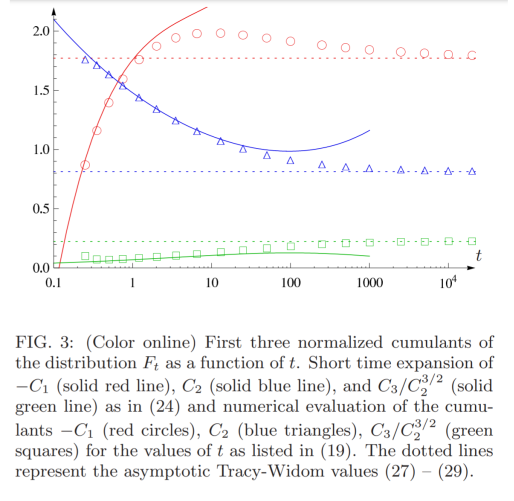
\includegraphics[width=8cm]{KPZGraph}
\caption{Variance of $\tilde{h}^{KPZ}(0, s)$ is in the blue triangles.}
\end{figure}

So now if we plug in $s$ and $x_{0}^{2}=\frac{2\log(N)}{t^{1/2}}$ into Equation 1 we get

\begin{equation}
\textbf{var}(Q_{B}(N, t)) = \textbf{var}(\tilde{h}^{KPZ}(0, \frac{4\log{N}^{2}}{t}))\frac{t^{1/2}t^{1/2}}{2\log(N)}
\end{equation}

Solving for $\textbf{var}(\tilde{h}^{KPZ}(0, \frac{\log{N}^{2}}{t}))$,

\begin{equation}
\textbf{var}(\tilde{h}^{KPZ}(0, \frac{4\log{N}^{2}}{t})) = \frac{2\log(N)}{t}\textbf{var}(Q_{B}(N, t))
\end{equation}

Then if we plot the RHS of Equation 3 on the y-axis and $\frac{4\log(N)^{2}}{t}$ on the x-axis we should
see the graph in Figure 1. Note that we aren't talking about the same time that is on the x-axis in Figure 1 since we want the plot of  $\textbf{var}(\tilde{h}^{KPZ}(0, \frac{4\log{N}^{2}}{t}))$. I think this is most likely where the issue lies.

\begin{figure}[h]
\centering
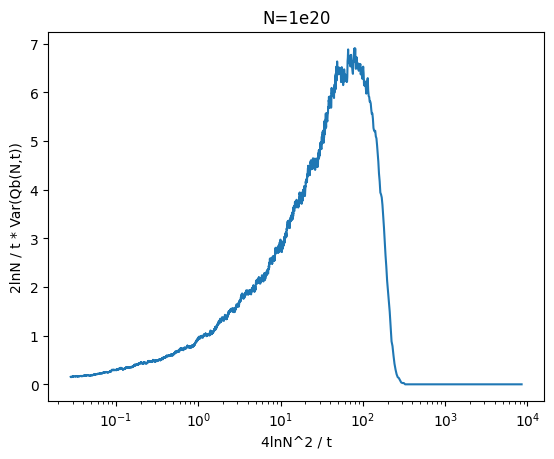
\includegraphics[width=8cm]{KPZVar1e20}
\caption{Calculated curve for $\tilde{h}^{KPZ}(0, s)$}
\end{figure}

\begin{figure}[h]
\centering
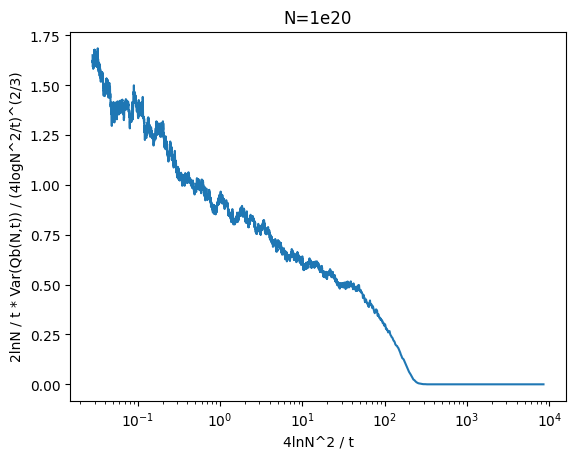
\includegraphics[width=8cm]{KPZVar1e20Scaled}
\caption{Calculated curve for $\tilde{h}^{KPZ}(0, s)$ but y-axis is scaled by $s^(2/3)$}
\end{figure}

The figure was generated using the PDF for ~1000 systems out to t=300,000 and for the 1e20 quantile. An interesting thing to note is that the graphs are not the same for different quantiles. Additonally, the unscaled variance is plotted in the figure below.

If there aren't any issues above, could there be an assumption that was made to get the $t^{1/2}$ scaling
that we need to do here. Such as it only holds for $t >> lnN^{2}$.

\begin{figure}[h]
\centering
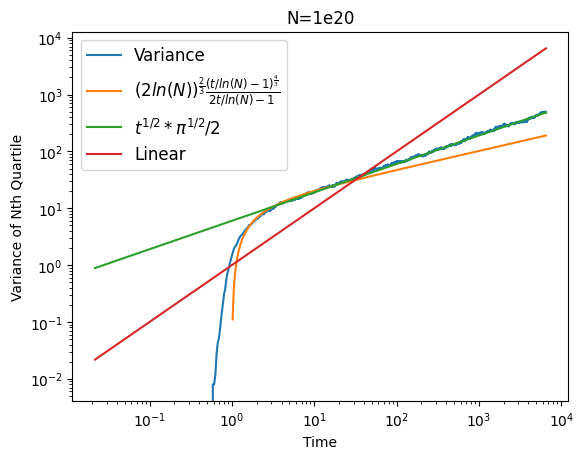
\includegraphics[width=8cm]{Var1e20}
\caption{Variance of the 1e20 quantile.}
\end{figure}

\end{document}
